\documentclass[11pt, oneside]{scrreprt}   	% use "amsart" instead of "article" for AMSLaTeX format
\usepackage{geometry}                		% See geometry.pdf to learn the layout options. There are lots.
\geometry{letterpaper}                   		% ... or a4paper or a5paper or ... 
%\geometry{landscape}                		% Activate for rotated page geometry
%\usepackage[parfill]{parskip}    		% Activate to begin paragraphs with an empty line rather than an indent
\usepackage{graphicx}				% Use pdf, png, jpg, or eps§ with pdflatex; use eps in DVI mode
								% TeX will automatically convert eps --> pdf in pdflatex		
\usepackage{amssymb}
\usepackage{amsmath,amsfonts,amsthm} % Math packages
\usepackage{bm}
\usepackage{subcaption}
%\usepackage{algorithm2e}
%\usepackage{algorithmic}
\usepackage{algorithm}
\usepackage[noend]{algpseudocode}
\usepackage{graphicx}
\graphicspath{ {images/} }

\makeatletter
\def\BState{\State\hskip-\ALG@thistlm}
\makeatother

%%%%%%%%
%    Cover     %
%%%%%%%%
\title{\textit{}\\\textit{}\\Time Series Analysis with\\ State Space Models}
\author{Hans-Peter H{\"o}llwirth}
\publishers{Master Project Report \\ 
Barcelona Graduate School of Economics \\ Master Degree in Data Science \\ 2017}
\date{}

\begin{document}
\maketitle
%\afterpage{\blankpage}

%%%%%%%%%%%%%
%    Table of Contents   %
%%%%%%%%%%%%%
\newpage
\setcounter{secnumdepth}{1}
\setcounter{tocdepth}{1}
\tableofcontents
\newpage

%%%%%%%%%%
%    Introduction   %
%%%%%%%%%%
\chapter{Introduction}
\label{chp:introduction}



%%%%%%%%
%    Models   %
%%%%%%%%
\chapter{State Space Models}
\label{chp:models}
State space models consist of two set of data:
\begin{enumerate}
	\item A series of \textbf{latent states} $\{x_t\}_{t=1}^T$ (with $x_t \in \mathcal{X}$) that forms a Markov chain. Thus, $x_t$ is independent of all past states but $x_{t-1}$.
	\item A set of \textbf{observations} $\{y_t\}_{t=1}^T$ (with $y_t \in \mathcal{Y}$) where any observation $y_t$ only depends on its latent state $x_t$. In other words, an observation is a noisy representation of its underlying state.
\end{enumerate}
Note that if the state space $\mathcal{X}$ and the observation state $\mathcal{Y}$ are both discrete sets, the state space model reduces to a Hidden Markov Model.\\

The relation between the latent states and observations can be summarized by two probability distributions:
\begin{enumerate}
	\item The \textbf{transition density} from the current state to a new state $p(x_{t+1} | x_t, \boldsymbol{\theta})$.
	\item The \textbf{measurement density} for an observation given the latent state $p(y_t | x_t, \boldsymbol{\theta})$.
\end{enumerate}
Here, $\boldsymbol{\theta} \in \Theta$ denotes the parameter vector of a state space model. 


%%%%  Local Level Model  %%%%
\section{Local Level Model}
Arguably, the simplest state space model is the (univariate) local level model. It has the following form:

\begin{center}
\begin{tabular}{ r r l }
  observation: & $y_t = x_t + \epsilon_t$, & $\epsilon_t \sim N(0,\sigma_{\epsilon}^2)$ \\
  state: & $x_{t+1} = x_t + \eta_t$, & $\eta_t \sim N(0,\sigma_{\eta}^2)$ \\
\end{tabular}
\end{center}
\bigskip
with some initial state $x_1 \sim N(\mu_1, \Sigma_1)$. All noise elements, i.e. all $\epsilon_t$'s and $\eta_t$'s, are both mutually independent and independent from the initial state $x_1$. Assuming that we know $\mu_1$ and $\Sigma_1$, the model is fully specified by the following vector of parameters:
$$
\boldsymbol{\theta} = [\sigma_{\eta}^2,  \sigma_{\epsilon}^2]^T
$$
Note that in the case of noise-free observations (i.e. $\sigma_{\eta}^2 = 0$), the model reduces to a pure random-walk. Likewise, if $\sigma_{\epsilon}^2 = 0$, the observations $\{y_t\}_{t=1}^T$ are a white noise representation of a some value $x_1$.\\
The transition and measurement density of the local level model are simple to deduce:
\begin{center}
\begin{tabular}{ r l }
  $p(x_{t+1} | x_t, \boldsymbol{\theta})$ & $\sim N(x_t,\sigma_{\epsilon}^2)$ \\
  $p(y_t | x_t, \boldsymbol{\theta})$ & $\sim N(x_t,\sigma_{\eta}^2)$ \\
\end{tabular}
\end{center}
\bigskip

%%%%  Latent State Inference  %%%%
\section{Latent State Inference}
Often, the main objective in state space models is to infer the latent state from observations. Let $\mathcal{I}_t$ denote the set of observed values up to time $t$:
$$
\mathcal{I}_t = \{y_1, y_2, \ldots, y_t\}
$$ 
Then information about the latent state $x_t$ can be summarized by the following two probability distributions:
\begin{enumerate}
	\item The \textbf{prediction density}, $p(x_{t} | \mathcal{I}_{t-1}, \boldsymbol{\theta})$, gives the probability of $x_t$ given past observations  $\mathcal{I}_{t-1}$.
	\item The \textbf{filtering density}, $p(x_{t} | \mathcal{I}_{t}, \boldsymbol{\theta})$, gives the probability of $x_t$ given the current and past observations  $\mathcal{I}_{t}$.
\end{enumerate}	
The prediction and filtering densities are recursively related. Given the filtering density for state $x_{t-1}$, the prediction density for state $x_t$ is
$$
p(x_{t} | \mathcal{I}_{t-1}, \boldsymbol{\theta}) = \int p(x_t | x_{t-1}, \boldsymbol{\theta}) p(x_{t-1} | \mathcal{I}_{t-1}, \boldsymbol{\theta}) dx_{t-1}
$$
where the first term in the integral is the transition density from $x_{t-1}$ to $x_t$, and the second term is the filtering density from before. Likewise, given the prediction density for state $x_t$, the filtering density for $x_t$ is
$$
p(x_{t} | \mathcal{I}_{t}, \boldsymbol{\theta}) \propto p(y_t | x_{t}, \boldsymbol{\theta}) p(x_{t} | \mathcal{I}_{t-1}, \boldsymbol{\theta}) 
$$

%%%%  Parameter Inference  %%%%
\section{Parameter Inference}
Assuming a particular state space model, another common objective is is to infer the model parameters from observations. This is usually achieved via \textbf{maximum likelihood estimation}. The log-likelihood of the observations for a given parameter vector $\boldsymbol{\theta}$ is the product of the conditional densities of observations, given all previous observations:
\begin{align} 
\begin{split}
\log \mathcal{L}(\boldsymbol{\theta}) &= \log \prod_{t=1}^T p(y_t | \mathcal{I}_{t-1}, \boldsymbol{\theta})\\
&= \sum_{t=1}^T \log  p(y_t | \mathcal{I}_{t-1}, \boldsymbol{\theta})\\
&= \sum_{t=1}^T \log  \int p(y_t | x_{t}, \boldsymbol{\theta}) p(x_{t} | \mathcal{I}_{t-1}, \boldsymbol{\theta}) d x_t\\
\end{split}					
\end{align} 
The decomposition of the observation densities into measurement density and prediction density, however, makes the maximization problem analytically intractable for most state space models.



%%%%%%%
%  Filtering %
%%%%%%%
\chapter{Filtering}
\label{chp:filtering}
% add parameter
The objective of filtering is to update our knowledge of the system each time a new observation $y_t$ is brought in. That is, we want to find an estimate of the latent process $x_{0:t}$, given all observations $\mathcal{I}_t = y_{0:t}$ and the model parameters $\boldsymbol{\theta}$:
$$
x_{0:t} | \mathcal{I}_t, \boldsymbol{\theta}
$$
Note that the joint distribution of the latent process conditioned on the observations can be decomposed in a recursive form:
$$
p(x_{0:t} | \mathcal{I}_t,\boldsymbol{\theta}) = \Big[ \frac{p(y_t | x_t,\boldsymbol{\theta}) p(x_t | x_{t-1},\boldsymbol{\theta})}{p(y_t | \mathcal{I}_{t-1},\boldsymbol{\theta})} \Big] p(x_{0:(t-1)} | \mathcal{I}_{t-1},\boldsymbol{\theta}) 
$$
This form allows for updating our knowledge of the system in an online fashion. This has significant computational advantages: We do not need to keep the whole time series in memory and we can simply update our knowledge once we observe a new $y_t$. Unfortunately, in many state space models the normalization term 
$$
p(y_t | \mathcal{I}_{t-1},\boldsymbol{\theta}) = \int p(y_t | x_t,\boldsymbol{\theta}) p(x_t | x_{t-1}, \boldsymbol{\theta}) d x_t
$$ 
is analytically intractable. One notable exception are linear Gaussian state space models such as the local level model.

%%%%  Kalman Filter   %%%%
\section{Kalman Filter}
State space models in which both the latent states $\{x_t\}_{t=1}^T$ and the observations $\{y_t\}_{t=1}^T$ have linear dependencies and are normally distributed, the joint distribution and of the latent process $p(x_{0:t} | y_{0:t})$ is also Gaussian (and so are the prediction and filtering density). 
The inference problem can be analytically solved by using standard results of multivariate Gaussian marginal and conditional distributions.\\

The \textit{Kalman filter}, however, uses a more efficient way to infer the latent states. 
The filter recursively computes the Gaussian prediction density $p(x_{t} | \mathcal{I}_{t-1}, \boldsymbol{\theta}) = N(\mu_{t | t-1}, \Sigma_{t | t-1})$ and filtering density $p(x_{t} | \mathcal{I}_{t}, \boldsymbol{\theta}) = N(\mu_{t | t}, \Sigma_{t | t})$ by obtaining their respective mean and covariance. 
This method has the big advantage that it does not need all observations to be kept in memory and can easily update the system whenever a new observation is made.
Consider the multivariate generalization of the univariate local level model from before:
\bigskip
\begin{center}
\begin{tabular}{ r r l }
  observation: & $\boldsymbol{y}_t = \boldsymbol{x}_t + \boldsymbol{\epsilon}_t$, & $\boldsymbol{\epsilon}_t \sim N(\textbf{0}, \Sigma_{\epsilon})$ \\
  state: & $\boldsymbol{x}_{t+1} = \boldsymbol{x}_t + \boldsymbol{\eta}_t$, & $\boldsymbol{\eta}_t \sim N(\textbf{0}, \Sigma_{\eta})$ \\
\end{tabular}
\end{center}
\bigskip
For the case of this model, the mean and (co)variance of the prediction and filtering density are updated as follows:
\begin{enumerate}
	\item The \textbf{prediction step} obtains the \textit{a priori} estimate of $\boldsymbol{x}_t$, given $\mathcal{I}_{t-1}$ (using the \textit{a posteriori} estimate with $t-1$).
		\begin{align} 
		\begin{split}
		\boldsymbol{\mu}_{t | t-1} &= \boldsymbol{\mu}_{t-1 | t-1}\\
		\Sigma_{t | t-1} &= \Sigma_{t-1 | t-1} + \Sigma_{\eta}\\
		\end{split}					
		\end{align} 
	\item The \textbf{update step} combines a new observation $\boldsymbol{y}_t$ with the \textit{a priori} estimate to obtain an improved \textit{a posteriori} estimate. 
		\begin{align} 
		\begin{split}
		\boldsymbol{\mu}_{t | t} &= \boldsymbol{\mu}_{t | t-1} + K_t \boldsymbol{v}_t\\
		\Sigma_{t | t} &= \Sigma_{t | t-1}(1 - K_t)\\
		\end{split}					
		\end{align} 
		where $\boldsymbol{v}_t = \boldsymbol{y}_t - \boldsymbol{\mu}_{t | t-1}$ denotes the difference between prediction and observation and $K_t = \Sigma_{t | t-1} (\Sigma_{t | t-1} + \Sigma_{\epsilon})^{-1}$ denotes the \textit{Kalman gain}. It determines how much the new observation affects the updated prediction.	
\end{enumerate}

%  Algorithm    %
\subsection{Algorithm}
Note that to start the recursion, we need an initial state density with $\boldsymbol{\mu}_1$ and $\Sigma_1$. In the following version of the algorithm we assume $\boldsymbol{\mu}_1$ and $\Sigma_1$ to be known. There are various ways to initialize the algorithm when $\boldsymbol{\mu}_1$ and $\Sigma_1$ are unknown, however, these methods are beyond the scope of this project.\\

\begin{algorithm}[h!]
\caption{(Local Level) Kalman filter}
\label{alg:kalman}
  \begin{algorithmic}[1]
    \Procedure{KalmanFilter}{$\mathcal{I}_T, \boldsymbol{\theta}, \boldsymbol{\mu}_1,\Sigma_1$}
      \smallskip
      \State $\boldsymbol{\mu}_{1 | 0}\gets \boldsymbol{\mu}_1$\Comment{initialization}
      \State $\Sigma_{1 | 0}\gets \Sigma_1$
      \smallskip
      \For{\texttt{$t$ in $1:T$}}
      	\State $\boldsymbol{v}_t = \boldsymbol{y}_t - \boldsymbol{\mu}_{t | t-1}$
      	\State $K_t = \Sigma_{t | t-1} (\Sigma_{t | t-1} + \Sigma_{\epsilon})^{-1}$
	\smallskip
      	\State $\boldsymbol{\mu}_{t | t} = \boldsymbol{\mu}_{t | t-1} + K_t \boldsymbol{v}_t$\Comment{update step}
      	\State $\Sigma_{t | t} = \Sigma_{t | t-1}(1 - K_t)$
	\smallskip
      	\State $\boldsymbol{\mu}_{t+1 | t}\gets \boldsymbol{\mu}_{t | t}$\Comment{prediction step}
      	\State $\Sigma_{t+1 | t}\gets \Sigma_{t | t} + \Sigma_{\eta}$
      \EndFor
      \State \textbf{return} $\{\boldsymbol{\mu}_{t | t}\}$, $\{\Sigma_{t | t}\}$
    \EndProcedure
  \end{algorithmic}
\end{algorithm}
\textit{Algorithm \ref{alg:kalman}} describes the recursive update of the prediction and filtering density.  For our purpose, the algorithm returns the filtering densities. 
The sequence of filtering means $\{\boldsymbol{\mu}_{t | t}\}$ is the best possible estimation for the latent states $\{\boldsymbol{x}_t\}$. 
The sequence of covariances $\{\Sigma_{t | t}\}$ can be used to obtain confidence intervals for these estimates. \\  

Note that the algorithm needs to invert the matrix $F_t = \Sigma_{t | t-1} + \Sigma_{\epsilon}$ at each iteration. For large dimensions of the states/observations, this can slow down this version of the Kalman filter significantly.

%  Example    %
\subsection{Example: Local Level Model}
\textit{Figure \ref{fig:ullm-kalman}} shows a realization of the univariate local level model with parameters $\sigma_{\eta}^2=1.4$ and $\sigma_{\epsilon}^2=1.0$ (left plot) and the Kalman prediction with a $95\%$ confidence level (right plot).
\begin{figure}[h!]
\centering
\begin{subfigure}{.5\textwidth}
  \centering
  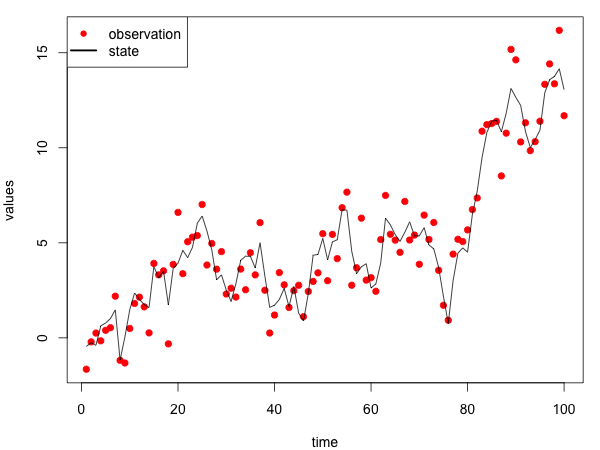
\includegraphics[width=75mm]{../../images/ullm-realization.png}
\end{subfigure}%
\begin{subfigure}{.5\textwidth}
  \centering
  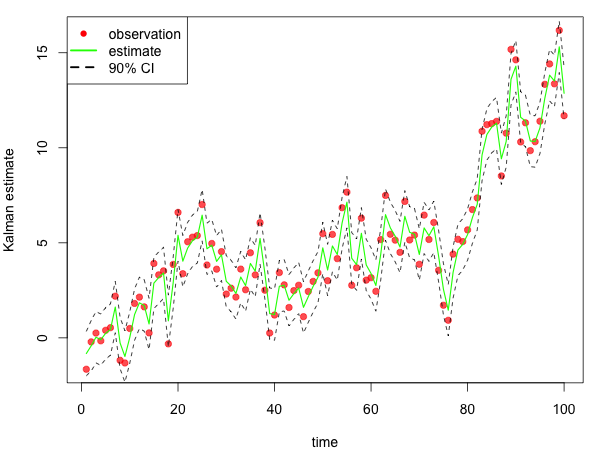
\includegraphics[width=75mm]{../../images/ullm-estimate-kalman.png}
\end{subfigure}
\caption{Kalman estimate of univariate local level realization}
\label{fig:ullm-kalman}
\end{figure}

%  Likelihood    %
\subsection{Likelihood evaluation}
The log-likelihood function for the linear Gaussian space model has the following (\textit{prediction error decomposition}) form:
$$
\log \mathcal{L}(\mathcal{I}_T, \boldsymbol{\theta}) = -\frac{Td}{2} \log(2 \pi) - \frac{1}{2} \sum_{t=1}^T (\log |F_t| + v_t^TF_t^{-1} v_t)
$$
Its elements $F_t$ and $v_t$ are routinely calculated by the Kalman filter and so the log-likelihood can be directly evaluated in the Kalman function. Note that $F_t$ might not be singular for all $t=1,\ldots, T$ for particular $\boldsymbol{\theta}$ values. Setting $\log \mathcal{L}(\mathcal{I}_T, \boldsymbol{\theta}) = -\infty$ in this case suffices for the purpose of maximum likelihood estimation.

%%%%  SIR Particle Filter   %%%%
\section{SIR Particle Filter}
If the state space model is not linear and Gaussian, both the joint distribution $p(x_{0:t} | \mathcal{I}_t)$ and the marginal distribution $p(x_{t} | \mathcal{I}_t)$ are usually not analytically solvable due to the intractability of the normalization constant $p(y_t | \mathcal{I}_{t-1})$. In this case we can only resort to sampling techniques to approximate these distribution densities. \\

\textit{Particle filtering} methods (which constitute a sub-class of \textit{Sequential Monto Carlo} methods) approximate the prediction density $p(x_{t} | \mathcal{I}_{t-1}, \boldsymbol{\theta})$ and filtering density $p(x_{t} | \mathcal{I}_{t}, \boldsymbol{\theta})$ sequentially by using importance sampling techniques. Many different method variants exist, all of which involve two basic steps: simulating from the transition density $p(x_{t+1} | x_t, \boldsymbol{\theta})$ and evaluating the measurement density $p(y_t | x_t, \boldsymbol{\theta})$. 

%  SIR    %
\subsection{Sequential Importance Resampling (SIR)}
One of the best-known particle filter methods is the \textit{Sequential Importance Resampling (SIR)} algorithm by Gordon et al. (1993). Let $P$ be the number of particles (= samples) per state. The algorithm recursively computes prediction and filtering particles:
\begin{enumerate}
	\item The \textbf{prediction step} obtains a new prediction particle for each filtering particle by propagating the system, using the transition density:
	$$
	x_{t | t-1}^i \sim p(x_t | x_{t-1 | t-1}^i, \theta) \quad \text{for } i=1, \ldots, P
	$$
	\item The \textbf{filtering step} (or update step) computes the importance weight $w_t^i$ of each prediction particle 
	$$
	w_{t}^i = \frac{p(y_t | x_{t | t-1}^i, \theta)}{\sum_{j=1}^P p(y_t | x_{t | t-1}^j, \theta)} \quad \text{for } i=1, \ldots, P
	$$
	and then picks the filtering particles via multinomial sampling, using the computed importance weights as respective probabilities:	
	$$
	x_{t | t }^j \sim MN(w_t^1, \ldots, w_t^P) \quad \text{for } j=1, \ldots, P
	$$
\end{enumerate}
The algorithm's main characteristic is the resampling within the filtering step which removes particles with small weights with high probability while likely copying particles with high weights multiple times. While this step increases the immediate Monte Carlo variance, it gives better stability for future steps by reducing the risk of weight degeneracy (Doucet and Johansen, 2008). 

%  Algorithm    %
\subsection{Algorithm}
In the following version of the algorithm we assume the initialization parameters $\boldsymbol{\delta}$ to be known. For example, in the case of the local level model, $\boldsymbol{\delta} = [\boldsymbol{\mu}_1, \Sigma_1]^T$.\\

\begin{algorithm}[h!]
\caption{Sequential Importance Sampling}
\label{alg:sir}
\begin{algorithmic}[1]
	\Procedure{SIR}{$\mathcal{I}_T, \boldsymbol{\theta}, \boldsymbol{\delta}, P$}
      	\smallskip
	\For{\texttt{$i$ in $1:P$}}
		\State $x_{0 | 0 }^i \sim p(x_{0 | 0 } | \boldsymbol{\delta})$ \Comment{initialization}
	\EndFor
      	\smallskip
      	\For{\texttt{$t$ in $1:T$}}
      		\For{\texttt{$i$ in $1:P$}}
      			\State $x_{t | t-1}^i \sim p(x_t | x_{t-1 | t-1}^i, \boldsymbol{\theta})$ \Comment{prediction step}
			\smallskip
      			\State $\tilde{w}_t^i \gets p(y_t | x_{t | t-1}^i, \boldsymbol{\theta})$ \Comment{compute importance weights}
		\EndFor	
		\smallskip
		\For{\texttt{$i$ in $1:P$}}
			\State $w_t^i \gets \tilde{w}_t^j / \sum_{j=1}^P \tilde{w}_t^j$ \Comment{normalize weights}
		\EndFor	
		\smallskip
		\For{\texttt{$i$ in $1:P$}}
			\State $x_{t | t }^i \sim MN(w_t^1, \ldots, w_t^P)$ \Comment{filtering step}
		\EndFor
      \EndFor
      \State \textbf{return} $\{\{\boldsymbol{x}_{t | t}^i\}_{i=1}^P\}_{t=1}^T$
    \EndProcedure
  \end{algorithmic}
\end{algorithm}
\textit{Algorithm \ref{alg:sir}} describes the recursive computation of the prediction and filtering particles.  
For our purpose, the algorithm returns the filtering particles which estimate the filtering density $p(x_t | \mathcal{I}_t, \boldsymbol{\theta})$ (for other purposes it could return the prediction particles instead). 
An estimate of the latent states can be constructed by averaging over the particles for each time $t$ with equal weights: 
$$
\hat{x}_t = \frac{1}{P}\sum_{i=1}^P x_{t | t}^i
$$
Their standard deviation (or other sample quantiles) can be used to construct confidence intervals for these estimates. 

The sequence of filtering means $\{\boldsymbol{\mu}_{t | t}\}$ is the best possible prediction for the latent states $\{\boldsymbol{x}_t\}$. 
The sequence of covariances $\{\Sigma_{t | t}\}$ can be used to obtain confidence intervals for these estimates. \\  

%  Example    %
\subsection{Example: Local Level Model}
In the case of the univariate local level model with $\boldsymbol{\theta}=[\sigma_{\eta}^2, \sigma_{\epsilon}^2]^T$, the prediction step draws from a normal transition density: $p(x_t | x_{t-1 | t-1}^i, \boldsymbol{\theta}) = N(x_{t-1 | t-1}, \sigma_{\eta}^2)$ and the importance weights are evaluated on a normal measurement density: $p(y_t | x_{t | t-1}^i, \boldsymbol{\theta}) = N(x_{t | t-1}, \sigma_{\epsilon}^2)$. The state initialization density is $p(x_{0 | 0 } | \boldsymbol{\delta}) = N(\mu_1, \Sigma_1)$.\\

\textit{Figure \ref{fig:ullm-particle}} shows the SIR particle filter estimate with $P=200$ particles for the same realization of the local level model that has been plotted in \textit{Figure \ref{fig:ullm-kalman}}. The left plot shows the estimated states together with the $0.05$ and $0.95$ sample quantiles. The right plot compares the SIR particle estimates with the Kalman estimates. 
\begin{figure}[h!]
\centering
\begin{subfigure}{.5\textwidth}
  \centering
  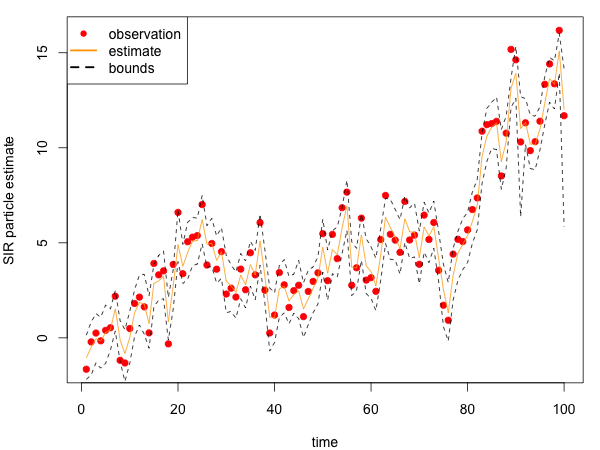
\includegraphics[width=75mm]{../../images/ullm-estimate-particle.png}
\end{subfigure}%
\begin{subfigure}{.5\textwidth}
  \centering
  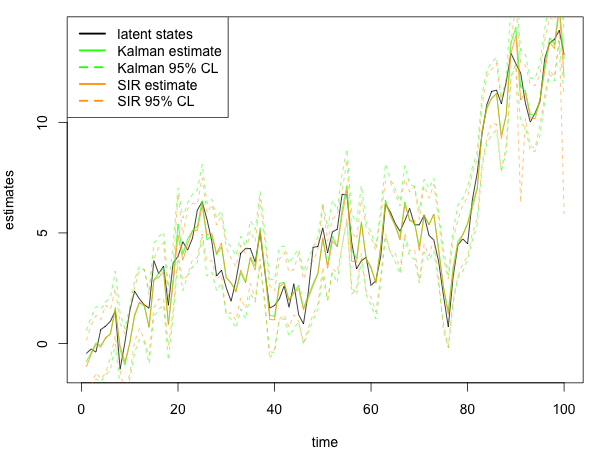
\includegraphics[width=75mm]{../../images/ullm-filter-comparison.png}
\end{subfigure}
\caption{SIR particle estimate of univariate local level realization}
\label{fig:ullm-particle}
\end{figure}
Note that the estimates of the Kalman filter and the SIR particle filter are almost identical. 
This is because the number of particles $P=200$ was chosen to be sufficiently large. 
In general, the approximation error of particle filter methods goes $0$ as $P \to \infty$.


%  Likelihood    %
\subsection{Likelihood evaluation}
The likelihood of a single observation given all previous observations $p(y_t | \mathcal{I}_{t-1}, \boldsymbol{\theta})$ can be estimated by simple Monte Carlo integration:
\begin{align} 
\begin{split}
p(y_t | \mathcal{I}_{t-1}, \boldsymbol{\theta}) &= \int p(y_t | x_t, \boldsymbol{\theta}) p(x_t | \mathcal{I}_{t-1}, \boldsymbol{\theta}) d x_t \\
\hat{p}(y_t | \mathcal{I}_{t-1}, \boldsymbol{\theta}) &\approx \frac{1}{P} \sum_{i=1}^P p(y_t | x_{t | t-1}^i, \boldsymbol{\theta})\\
 &= \frac{1}{P} \sum_{i=1}^P \tilde{w}_t^i\\
\end{split}					
\end{align}
Thus, the likelihood can be easily constructed from the (unnormalized) importance weights in the particle filter. The estimated log-likelihood of the whole system, described the the series of observations $\mathcal{I}_T$, can then be defined as
\begin{align} 
\begin{split}
\log \hat{\mathcal{L}}(\mathcal{I}_T, \boldsymbol{\theta}) &= \log \prod_{t=1}^T \hat{p}(y_t | \mathcal{I}_{t-1}, \boldsymbol{\theta}) \\
&= \sum_{t=1}^T \log \hat{p}(y_t | \mathcal{I}_{t-1}, \boldsymbol{\theta}) \\
&= \sum_{t=1}^T \log \frac{1}{P} \sum_{i=1}^P p(y_t | x_{t | t-1}^i, \boldsymbol{\theta}) \\
\end{split}					
\end{align} 
Note that for the sequential importance resampling algorithm, this log-likelihood estimator is not necessarily smooth with respect to $\boldsymbol{\theta}$. This can cause problems when trying to find the maximum like-likelihood. For this reason, \textit{Continuous Sequential Importance Sampling (CSIR)} proves to be a better algorithm for parameter inference.

%%%%  Importance Sampling Particle Filter   %%%%
\section{Importance Sampling Particle Filter}
The SIR algorithm suffers from not being necessarily smooth with respect to the model parameters $\boldsymbol{\theta}$ which makes the method unfit for parameter inference. The alternative continuous SIR algorithm smoothes the log-likelihood with respect to $\boldsymbol{\theta}$, however, the algorithm only works in the univariate case. For this reason, Brownlees and Kristensen (2017) propose a novel particle filter method called \textit{importance sampling particle filter} which smoothes the log-likelihood with respect to $\boldsymbol{\theta}$ and still works in the multivariate case. \\

The key idea of this new method is the following: Use an auxiliary, misspecified particle filter which does not depend on the model parameters $\boldsymbol{\theta}$ to compute the log-likelihood with respect to $\boldsymbol{\theta}$ via recursive importance sampling. Let $\tilde{p}(y_t | \tilde{x}_{t})$ be the auxiliary measurement density, let $\tilde{p}(\tilde{x}_{t+1} | \tilde{x}_{t})$ be the auxiliary transition density, and let $\tilde{p}(\tilde{x}_1)$ be the auxiliary initial density. Furthermore, let $\tilde{p}(\tilde{x}_{t} | \mathcal{I}_{t-1})$ and  $\tilde{p}(\tilde{x}_{t} | \mathcal{I}_{t})$ be the auxiliary prediction and filtering density, respectively (note that none of those densities depends on the model parameter $\boldsymbol{\theta}$).\\

We can use the samples from the misspecified, auxiliary prediction distribution 
\begin{align} 
\begin{split}
p(y_t | \mathcal{I}_{t-1}, \boldsymbol{\theta}) &= \int p(y_t | \tilde{x}_t, \boldsymbol{\theta}) p(\tilde{x}_t | \mathcal{I}_{t-1}, \boldsymbol{\theta}) d \tilde{x}_t \\
&= \int p(y_t | \tilde{x}_t, \boldsymbol{\theta}) \bigg[ \frac{p(\tilde{x}_t | \mathcal{I}_{t-1}, \boldsymbol{\theta})}{p(\tilde{x}_t | \mathcal{I}_{t-1})} \bigg] p(\tilde{x}_t | \mathcal{I}_{t-1}) d \tilde{x}_t \\
\end{split}					
\end{align}  

%  Algorithm    %
\subsection{Algorithm}
\textit{Algorithm \ref{alg:is}} takes the predictive and filter particles of a misspecified model with parameter vector $\boldsymbol{\tilde{\theta}}$ as input. That means that we can run the sequential importance sampling (SIR) algorithm with any sensible choice of parameter values $\boldsymbol{\tilde{\theta}}$ and keep its predictive and filter particles to use them as input to the importance sampling particle filter. Note that the algorithm does not work with particles produced from the continuous sequential importance sampling (CSIR) algorithm.\\

\begin{algorithm}[h!]
\caption{Importance Sampling Particle Filter}
\label{alg:is}
\begin{algorithmic}[1]
	\Procedure{ISParticleFilter}{$\mathcal{I}_T, \{\{\boldsymbol{\tilde{x}}_{t | t}^i\}_{i=1}^P\}_{t=1}^T, \{\{\boldsymbol{\tilde{x}}_{t | t-1}^i\}_{i=1}^P\}_{t=1}^T, \boldsymbol{\theta}, \boldsymbol{\tilde{\theta}}$}
      	\smallskip
	\State $loglik \gets 0$
	\For{\texttt{$i$ in $1:P$}}
		\State $is_{1 | 0 }^i \gets p(\tilde{x}_{1 | 0 } | \boldsymbol{\theta}) / p(\tilde{x}_{1 | 0 } | \boldsymbol{\tilde{\theta}})$ \Comment{initialize predictive importance weights}
	\EndFor
      	\smallskip
      	\For{\texttt{$t$ in $1:T$}}
		\State $w_t \gets \tilde{w}_t \gets 0$
      		\For{\texttt{$i$ in $1:P$}} \Comment{estimate likelihoods}
      			\State $w_t \gets \tilde{w} + p(y_t | \tilde{x}_{t | t-1}^i, \boldsymbol{\theta})is_{t | t-1 }^i / P$ 
      			\State $\tilde{w}_t \gets \widehat{\tilde{w}} + p(y_t | \tilde{x}_{t | t-1}^i, \boldsymbol{\tilde{\theta}}) / P$ 
		\EndFor	
		\State $loglik \gets loglik + \log w_t$
		\smallskip
		\For{\texttt{$i$ in $1:P$}} \Comment{update filtering importance weights}
			\State $f \gets p(y_t | \tilde{x}_{t | t}^i, \boldsymbol{\theta})$ 
			\State $\tilde{f} \gets p(y_t | \tilde{x}_{t | t}^i, \boldsymbol{\tilde{\theta}})$ 
			\smallskip
			\State $is_{t | t }^i \gets (\tilde{w}_t / w_t) (f / \tilde{f}) is_{t | t-1 }^j$ \Comment{where $j$ is such that $\tilde{x}_{t | t}^i = \tilde{x}_{t | t-1}^j$}
		\EndFor	
		\smallskip
		\If{$t < T$}
			\For{\texttt{$i$ in $1:P$}} \Comment{update predictive importance weights}
				\State $p \gets p(\tilde{x}_{t+1 | t } | \tilde{x}_{t | t }, \boldsymbol{\theta})$ 
				\State $\tilde{p} \gets p(\tilde{x}_{t+1 | t } | \tilde{x}_{t | t }, \boldsymbol{\tilde{\theta}}) $ 
				\smallskip
				\State $is_{t+1 | t }^i \gets (p / \tilde{p}) is_{t | t }^i$ 
			\EndFor
		\EndIf
      \EndFor
      \smallskip
      \State \textbf{return} $loglik$
    \EndProcedure
  \end{algorithmic}
\end{algorithm}
Importantly, the algorithm does not produce any estimates or predictions on the latent states. The only object of interest the algorithm returns is the (log-)likelihood of the model with $\boldsymbol{\theta}$. This allows us to use the algorithm for parameter inference where it smoothes the (log-)likelihood with respect to $\boldsymbol{\theta}$. The algorithm can not be used for latent state inference.

%  Example    %
\subsection{Example: Local Level Model}
We consider the realization of an univariate local model with parameters plotted in \textit{Figure \ref{fig:ullm-kalman}} and take as input the filtering and prediction particles produced by the SIR algorithm whose latent state estimates have been plotted in \textit{Figure \ref{fig:ullm-particle}}. Note again that the importance sampling particle filter does not produce estimates of the latent state.\\

\textit{Figure \ref{fig:ullm_is-particle}} shows the mean filtering and predictive importance weights when we run the importance sampling particle filter with the true parameters $\boldsymbol{\theta} = [\sigma_{\eta}^2=1.4, \sigma_{\epsilon}^2=1.0]^T$, using auxiliary parameters $\boldsymbol{\tilde{\theta}} = [\tilde{\sigma}_{\eta}^2=1.0, \tilde{\sigma}_{\epsilon}^2=1.0]^T$. Observe that the weights all stay in a rather narrow bandwidth around 1. Note that the importance weights are all necessarily exactly $1$ if $\boldsymbol{\theta}=\boldsymbol{\tilde{\theta}}$.

\begin{figure}[h!]
\centering
\begin{subfigure}{1\textwidth}
  \centering
  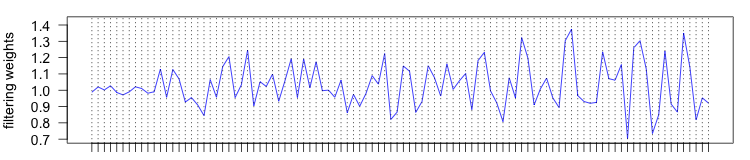
\includegraphics[width=150mm]{../../images/ullm_is_filt_weights_P200.png}
\end{subfigure}%
\\
\begin{subfigure}{1\textwidth}
  \centering
  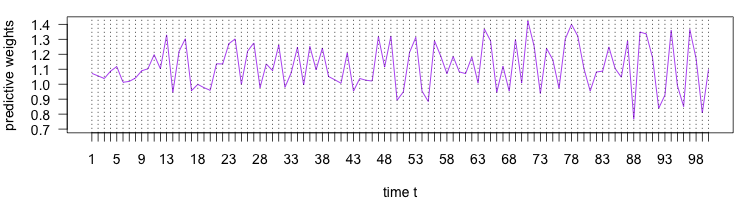
\includegraphics[width=150mm]{../../images/ullm_is_pred_weights_P200.png}
\end{subfigure}
\caption{Importance weights with $P=200$ particles}
\label{fig:ullm_is-particle}
\end{figure}


%  Likelihood    %
\subsection{Likelihood evaluation}
% add CSIR?
As explained earlier, the likelihood is directly evaluated by the importance sampling particle filter algorithm and is actually its main output. 
The algorithm approximates the log-likelihood via importance sampling. 
Its main attractive feature is that the log-likelihood is smooth with respect to $\boldsymbol{\theta}$. 
That claim is supported by the plots in in \textit{Figure \ref{fig:ullm_loglik}} which compare the log-likelihood of different methods for different values of $\sigma_{\eta}^2$ as $\sigma_{\epsilon}^2$ is kept at its true value ($1.0$): the Kalman filter (green), the SIR particle filter (orange), and the importance sampling particle filter (magenta).\\ 

\begin{figure}[h!]
\centering
\begin{subfigure}{0.5\textwidth}
  \centering
  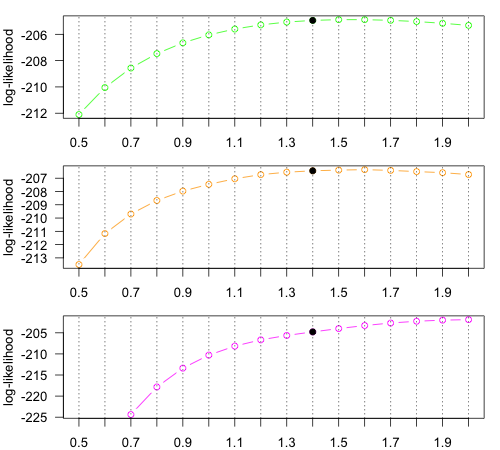
\includegraphics[width=75mm]{../../images/ullm-loglik-eta.png}
\end{subfigure}%
\begin{subfigure}{0.5\textwidth}
  \centering
  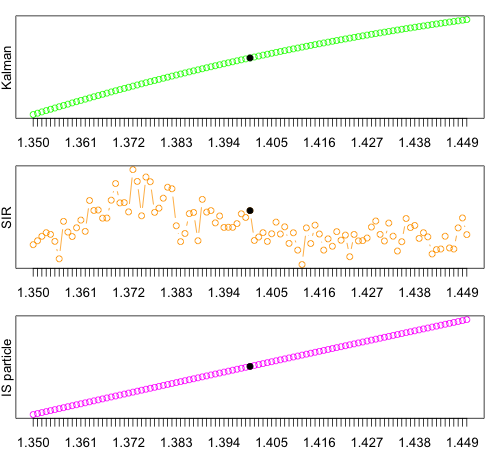
\includegraphics[width=75mm]{../../images/ullm-loglik-detail.png}
\end{subfigure}
\caption{Log-likelihood as a function of $\sigma_{\eta}^2$ with different filters}
\label{fig:ullm_loglik}
\end{figure}

The left plots show the log-likelihood for larger step sizes ($0.1$) of $\sigma_{\eta}^2$. The function with respect to $\sigma_{\eta}^2$ appears to be smooth for all three filters. However, as the right plots show, the picture changes when we decrease the step size to $0.001$ around the true $\sigma_{\eta}^2$. While both the Kalman and the IS particle filter still produce a smooth, concave log-likelihood curve, the log-likelihood plot of the SIR particle filter reveals many local optima. The log-likelihood for the true parameter $\sigma_{\eta}^2 = 1.4$ is highlighted with a black point.\\   

\begin{figure}[h!]
\centering
\begin{subfigure}{0.5\textwidth}
  \centering
  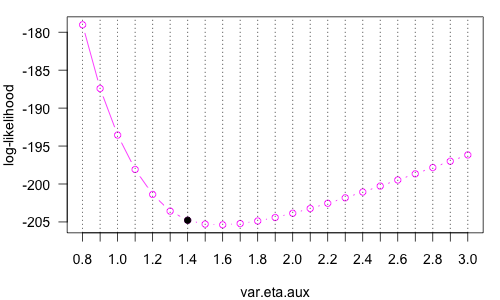
\includegraphics[width=75mm]{../../images/ullm-loglik-aux-eta.png}
\end{subfigure}%
\begin{subfigure}{0.5\textwidth}
  \centering
  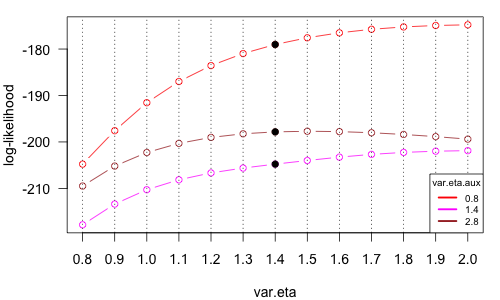
\includegraphics[width=75mm]{../../images/ullm-loglik-aux-eta-2.png}
\end{subfigure}
\caption{Impact of choice of $\tilde{\sigma}_{\eta}^2$ on log-likelihood of IS particle filter}
\label{fig:ullm_theta_aux}
\end{figure}

In the simulation of the importance sampling particle filter, the auxiliary parameters $\boldsymbol{\tilde{\theta}}=[\tilde{\sigma}_{\eta}^2, \tilde{\sigma}_{\epsilon}^2]^T$ have been set to the true parameters $\tilde{\sigma}_{\eta}^2=1.4$ and $\tilde{\sigma}_{\epsilon}^2=1.0$. \textit{Figure \ref{fig:ullm_theta_aux}} shows how the choice of the auxiliary parameters impact the log-likelihood values of the IS particle filter. The left plot shows the log-likelihood evaluated for the true parameters as a function of the auxiliary parameter $\tilde{\sigma}_{\eta}^2$ (meanwhile, $\tilde{\sigma}_{\epsilon}^2$ is kept fixed at $\sigma_{\epsilon}^2=1.0$). The log-likelihood is smallest close to $\tilde{\sigma}_{\eta}^2=\sigma_{\eta}^2=1.4$ and smoothly increases as $\tilde{\sigma}_{\eta}^2$ moves further away. The graph shows that the value of the log-likelihood of the IS particle filter depends on the choice of the auxiliary parameters.\\

The right graph in \textit{Figure \ref{fig:ullm_theta_aux}} plots the log-likelihood for the same filtering and predictive particles as a function of $\sigma_{\eta}^2$ for 3 choices of $\tilde{\sigma}_{\eta}^2$: $0.8$, $1.4$, and $2.8$. We see that the shape of the curves are similar (in particular, concave), but do not peak at the same value of $\sigma_{\eta}^2$. 

%%%%%%%%%%
%    Evaluation   %
%%%%%%%%%%
\chapter{Evaluation}
\label{chp:evaluation}

%%%%  Comparison  %%%%
\section{Method Comparison}
\textit{Table \ref{tab:filter_summary}} summarizes for which models and inference types the presented filters can be potentially used. \\

\begin{table}[h!]
\centering
\begin{tabular}{lccl}
\hline
Filter  & Latent state & Parameter & Comment\\
\hline
Kalman    & x & x & linear Gaussian models only\\
SIR      & x & &\\
CSIR      & x & x & univariate models only\\
IS      & & x & \\
\hline
\end{tabular}
\caption{Summary of inference with presented filters}
\label{tab:filter_summary}
\end{table}

The Kalman filter only works for linear Gaussian state space models. Kalman's latent state estimates statistically minimize the error and so is optimal with respect to many different statistical measures, eg. the mean squared error.  The sequential importance resampling (SIR) particle filter works for latent state inference but usually performs poorly for parameter inference where the log-likelihood with respect to the parameters lacks smoothness. The continuous SIR method smoothes the log-likelihood with respect to the parameters and so works for both latent state and parameter inference. However, CIR only applies to univariate models. Finally, the novel importance sampling particle filter solves parameter inference for any type of state space models. The method does not produce any filtering or prediction particles though and so cannot be used for latent state inference. 


%%%%  Parameter Inference  %%%%
\section{Parameter Inference}
In this section we compare the performance on parameter inference with respect to bias, standard error, and mean squared error (MSE) for the maximum likelihood estimator (MLE) of different filters. We test the performance on random realizations of the univariate local level model with $\sigma_{\eta}^2=1.4$ and $\sigma_{\epsilon}^2=1.0$ of several different lengths $T$. The CSIR method and the importance sampling particle filter are tested for different particle sizes $P$.

%bias
\begin{table}[h!]
\centering
\begin{tabular}{rrrrrrrrrr}
\hline
T  & Kalman &  \multicolumn{3}{c}{CSIR} &  \multicolumn{3}{c}{IS}\\
\cline{3-8}
& & P50 & P200 & P500 & P50 & P200 & P500\\
\hline
50        & -0.053 & P50 & P200 & P500 & P50 & P200 & P500\\
100      & -0.103 & P50 & P200 & P500 & P50 & P200 & P500\\
250      & -0.089 & P50 & P200 & P500 & P50 & P200 & P500\\
500      & -0.085 & P50 & P200 & P500 & P50 & P200 & P500\\
\hline
\end{tabular}
\caption{Monte Carlo bias summary}
\label{tab:param_inference_bias}
\end{table}

\textit{Table \ref{tab:param_inference_mse}} shows the bias results over $1000$ Monte Carlo simulations.

%standard error
\begin{table}[h!]
\centering
\begin{tabular}{rrrrrrrrrr}
\hline
T  & Kalman &  \multicolumn{3}{c}{CSIR} &  \multicolumn{3}{c}{IS}\\
\cline{3-8}
& & P50 & P200 & P500 & P50 & P200 & P500\\
\hline
50        & 0.057 & P50 & P200 & P500 & P50 & P200 & P500\\
100      & 0.036 & P50 & P200 & P500 & P50 & P200 & P500\\
250      & 0.023 & P50 & P200 & P500 & P50 & P200 & P500\\
500      & 0.017 & P50 & P200 & P500 & P50 & P200 & P500\\
\hline
\end{tabular}
\caption{Monte Carlo standard error summary}
\label{tab:param_inference_se}
\end{table}

%MSE
\begin{table}[h!]
\centering
\begin{tabular}{rrrrrrrrrr}
\hline
T  & Kalman &  \multicolumn{3}{c}{CSIR} &  \multicolumn{3}{c}{IS}\\
\cline{3-8}
& & P50 & P200 & P500 & P50 & P200 & P500\\
\hline
50        & 0.322 & P50 & P200 & P500 & P50 & P200 & P500\\
100      & 0.141 & P50 & P200 & P500 & P50 & P200 & P500\\
250      & 0.059 & P50 & P200 & P500 & P50 & P200 & P500\\
500      & 0.035 & P50 & P200 & P500 & P50 & P200 & P500\\
\hline
\end{tabular}
\caption{Monte Carlo MSE summary}
\label{tab:param_inference_mse}
\end{table}

%Conclusion: Particle filtering suffers from propagation error. Current approximations errors are related to past approximation errors. The number of particles $P$ should increase with the sample size $T$ to guarantee a good degree of approximation.


%%%%%%%%
%  Illustration %
%%%%%%%%
\chapter{Illustration}
\label{chp:Illustration}


%%%%  Trivariate Local Level Model  %%%%
\section{Trivariate Local Level Model}

\subsection{The Model}
Consider a time series of length $T$ with each observation $\boldsymbol{y}_t=[y_{1t}, y_{2t}, y_{3t}]^T$ and each state $\boldsymbol{x}_t=[x_{1t}, x_{2t}, x_{3t}]^T$ being described by a 3-dimensional vector.

\bigskip
\begin{center}
\begin{tabular}{ r r l }
  observation: & $\boldsymbol{y}_t = \boldsymbol{x}_t + \boldsymbol{\epsilon}_t$, & $\boldsymbol{\epsilon}_t \sim N(\textbf{0}, \sigma_{\epsilon}^2 I_3)$ \\
  state: & $\boldsymbol{x}_{t+1} = \boldsymbol{x}_t + \boldsymbol{\eta}_t$, & $\boldsymbol{\eta}_t \sim N(\textbf{0}, \Sigma_{\eta})$ \\
\end{tabular}
\end{center}
\bigskip
with initial state $\boldsymbol{x}_1 \sim N(\boldsymbol{\mu}_1, \Sigma_1)$ and where we restrict the covariance matrix of the state disturbances, $\Sigma_{\eta}$, to the form
$$
\Sigma_{\eta} = 
\begin{bmatrix}
\sigma_{\eta 1}^2 & \rho \sigma_{\eta 1} \sigma_{\eta 2} & \rho \sigma_{\eta 1} \sigma_{\eta 3}
\\ \rho \sigma_{\eta 1} \sigma_{\eta 2} & \sigma_{\eta 2}^2 & \rho \sigma_{\eta 2} \sigma_{\eta 3}
\\ \rho \sigma_{\eta 1} \sigma_{\eta 3} & \rho \sigma_{\eta 2} \sigma_{\eta 3} & \sigma_{\eta 3}^2
\end{bmatrix}
$$
Thus, $\Sigma_{\eta}$ can be described by $\sigma_{\eta 1}^2$, $\sigma_{\eta 2}^2$, $\sigma_{\eta 3}^2 > 0$ and $\rho \in [0,1]$. Furthermore, we assume for simplicity that the observation noise has the same variance in each dimension $\sigma_{\epsilon}^2 > 0$. Therefore, the model is fully specified by the following vector of parameters:
$$
\boldsymbol{\theta} = [\rho, \sigma_{\eta 1}^2, \sigma_{\eta 2}^2, \sigma_{\eta 3}^2, \sigma_{\epsilon}^2]^T
$$
The initial state parameters $\boldsymbol{\mu}_1$ and $\Sigma_1$ are assumed to be known.

\subsection{Realization}
\textit{Figure \ref{fig:mllm_realization}} plots the states and observations for a realization of the trivariate local level model with length $T=100$. The model parameters are 
$$
\boldsymbol{\theta} = [\rho = 0.7, \sigma_{\eta 1}^2 = 4.2, \sigma_{\eta 2}^2 = 2.8, \sigma_{\eta 3}^2 = 0.9, \sigma_{\epsilon}^2 = 1.0]^T
$$
The initial state $x_1$ is drawn from a standard normal.

\begin{figure}[h!]
\centering
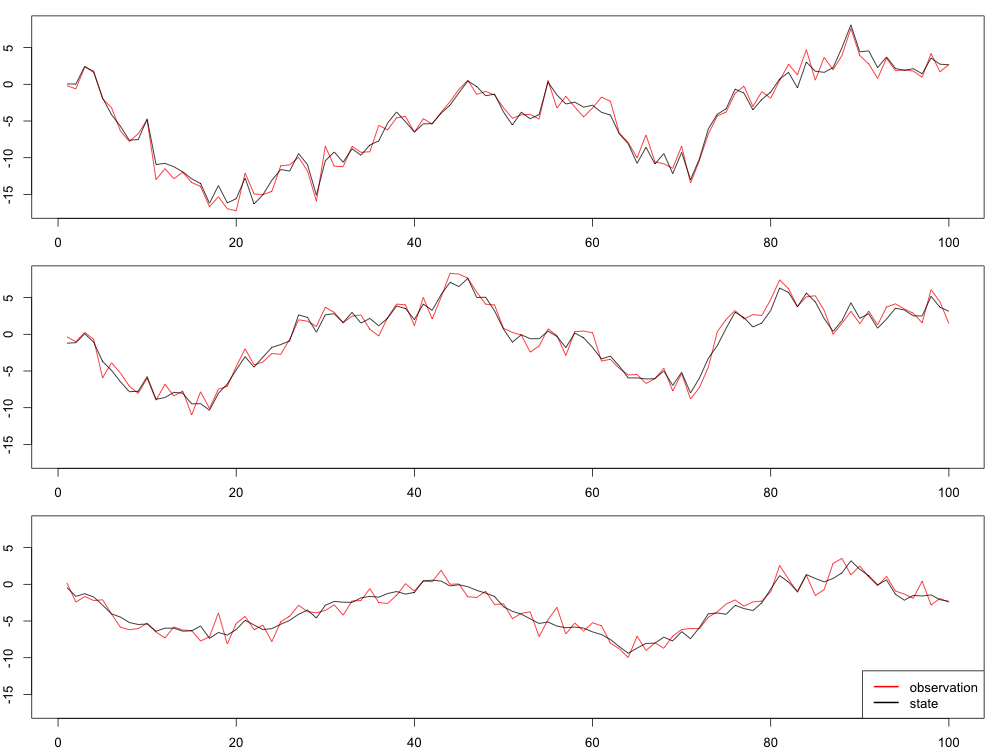
\includegraphics[width=115mm]{../../images/mllm-realization.png}
\caption{Realization of the model with $T=100$}
\label{fig:mllm_realization}
\end{figure}

%  Latent State Inference    %
\subsection{Latent State Inference}


%%%%  Hierarchical Dynamic Poisson Model   %%%%
\newpage
\section{Hierarchical Dynamic Poisson Model}
Next, we test the particle filters on a non-linear model with non-Gaussian observations, called \textit{hierarchical dynamic Poisson model}. The observations are modeled as a Poisson random variable and represent counts, i.e. the total number of occurrences during a fixed time period. The underlying latent state of an observation is modeled as the the average number of counts in that interval (i.e. the state is the parameter of the Poisson distribution). The state is assumed to be constructed from 3 components: a daily level, intra-daily periodic changes, and intra-daily fluctuations. Both the daily level and intra-daily fluctuations are are assumed to form an (independent) Markov chain. The model in this form might be well suited to model demand in various settings such as server access or patients in a hospital.

%  Model    %
\subsection{The Model}
Consider a time series over $M$ days, each consisting of $N$ intra-daily observations. 
Let $m$ denote the day and $n$ be the intraday index.

\bigskip
\begin{center}
\begin{tabular}{ r r l }
  observation: & $y_{m,n}$ & $\sim \text{Poisson}(\lambda_{m,n})$\\
  state: & $\log \lambda_{m,n}$ & $= \log \lambda_m^{(D)} + \log \lambda_{m,n}^{(I)} + \log \lambda_n^{(P)}$\\  
\end{tabular}
\end{center}
\bigskip
where the state consists of a daily, an intra-daily, and a periodic component:
\bigskip
\begin{center}
\begin{tabular}{ r l l l}
  daily: & $\log \lambda_{m+1}^{(D)}$ &$= \phi_0^{(D)} + \phi_1^{(D)} \log \lambda_{m}^{(D)}  + \eta_m^{(D)}$ & $\eta_t \sim N(0, \sigma^2_{(D)})$ \\
  intra-daily: & $\log \lambda_{m,n+1}^{(I)}$ &$= \phi_1^{(I)} \log \lambda_{m,n}^{(I)}  + \eta_{m,n}^{(I)}$ & $\eta_{m,n} \sim N(0, \sigma^2_{(I)})$ \\
    periodic: & $\log \lambda_n^{(P)} $ &$= \phi_1^{(P)} \sin(\pi (n-1)/M)$ &\\
\end{tabular}
\end{center}
\bigskip
The initial daily and intra-daily component is drawn from a normal with mean $\mu_1$ and covariance $\Sigma_1$: 
$$\log \lambda_{1}^{(D)}, \log \lambda_{1}^{(I)}  \sim N(\mu_1, \Sigma_1)$$ 
Note that both the daily and intra-daily component constitute an AR(1) model, with the mean of the intra-daily component $\phi_0^{(I)}$ set to 0. 
The model is fully specified by the following vector of parameters:
$$
\boldsymbol{\theta} = [ \phi_0^{(D)},  \phi_1^{(D)}, \sigma^2_{(D)}, \phi_1^{(I)}, \sigma^2_{(I)}, \phi_1^{(P)}]^T
$$
Again, the initial state parameters $\mu_1$ and $\Sigma_1$ are assumed to be known.

%  Model Densities    %
\subsection{Model Densities}
The transition and measurement density of the hierarchical dynamic Poisson model can be described as a function of the state components:
\begin{center}
\begin{tabular}{ r l }
  $p(\log \lambda_{m,n+1} | \log \lambda_{m}^{(D)}, \log \lambda_{m,n}^{(I)}, \log \lambda_n^{(P)},\boldsymbol{\theta})$ & $\sim N(\mu_{m,n}, \sigma_{m,n}^2)$ \\
  $p(y_{m,n} | \log \lambda_{m}^{(D)}, \log \lambda_{m,n}^{(I)}, \log \lambda_n^{(P)},\boldsymbol{\theta})$ & $\sim \text{Poisson}(\lambda_{m}^{(D)} \lambda_{m,n}^{(I)} \lambda_n^{(P)})$ \\
\end{tabular}
\end{center}
where 
\begin{center}
\begin{tabular}{ r l }
  $\mu_{m,n}$ &= $\phi_0^{(D)} + \phi_1^{(D)} \log \lambda_{m}^{(D)} + \phi_1^{(I)} \log \lambda_{m,n}^{(I)} + \phi_1^{(P)} \sin(\pi (n-1)/M)$ \\
  $\sigma_{m,n}^2$ &= $\sigma_{(D)}^2 + \sigma_{(I)}^2$ \\
\end{tabular}
\end{center}
The transition and measurement density are used in the implementation of the SIR algorithm and the importance sampling particle filter.

%  Realization    %
\subsection{Realization}
The left graph in \textit{Figure \ref{fig:hdpm_realization}} plots the states and observations for a realization of the hierarchical dyanmic Poisson model over $N=5$ days with $M=20$ intra-daily observations. The model parameters are 
$$
\boldsymbol{\theta} = [ \phi_0^{(D)} = 0.7,  \phi_1^{(D)} = 0.6, \sigma^2_{(D)} = 0.6, \phi_1^{(I)} = 0.3, \sigma^2_{(I)} = 0.2, \phi_1^{(P)} = 0.8]^T
$$
The initial daily and intra-daily state components were drawn from a standard normal. The right graph in \textit{Figure \ref{fig:hdpm_realization}} plots the state components $\log \lambda_{m}^{(D)}$, $\log \lambda_{m,n}^{(I)}$, and $\log \lambda_n^{(P)}$ of that realization.\\

\begin{figure}[h!]
\centering
\begin{subfigure}{.5\textwidth}
  \centering
  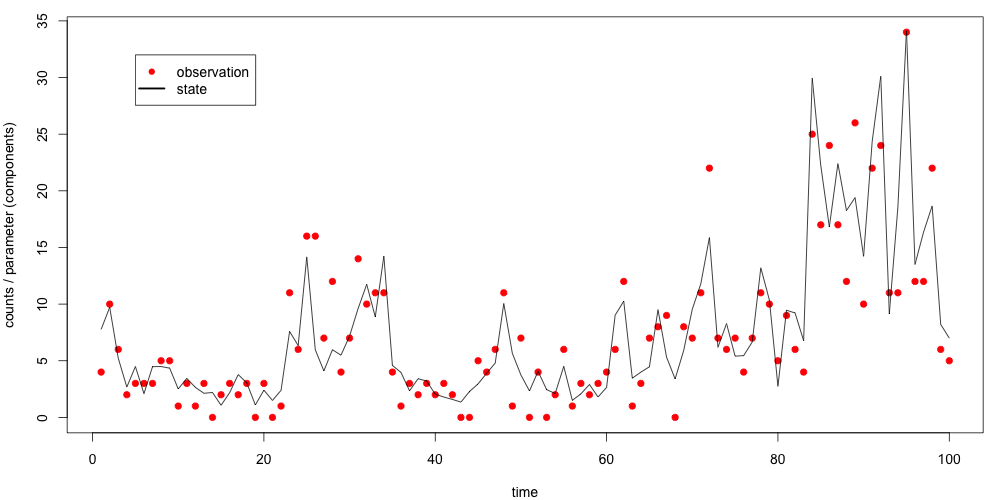
\includegraphics[width=73mm]{../../images/hdpm-realization.png}
\end{subfigure}%
\begin{subfigure}{.5\textwidth}
  \centering
  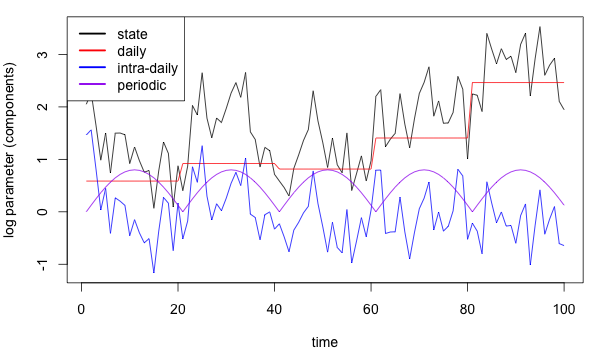
\includegraphics[width=73mm]{../../images/hdpm-log-param.png}
\end{subfigure}
\caption{Realization of the model with $N=5$ and $M=20$}
\label{fig:hdpm_realization}
\end{figure}

%  Latent State Inference    %
\subsection{Latent State Inference}
We estimate the latent state of the realization in \textit{Figure \ref{fig:hdpm_realization}} with the implementation of the sequential importance resampling (SIR) algorithm which uses the transition and measurement densities we derived before. The estimates of the latent states, together with the $90\%$ confidence interval (estimated by the $5\%$ and $95\%$ quantile of the $P=200$ particles) are plotted in \textit{Figure \ref{fig:hdpm_est}}.

\begin{figure}[h!]
\centering
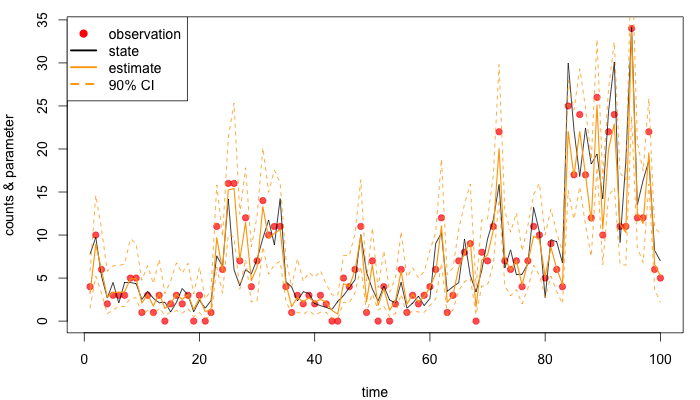
\includegraphics[width=115mm]{../../images/hdpm-est.png}
\caption{State estimates with SIR filter ($P=200$)}
\label{fig:hdpm_est}
\end{figure}

Note that neither the Kalman filter nor the continuous SIR method can be used for this model. The Kalman filter cannot be used because the model is non-linear (and the observations are not Gaussian). The continuous SIR particle filter is not applicable because the state is a multivariate variable, consisting of the daily, intra-daily, and periodic component.\\

%  Parameter Inference    %
\subsection{Parameter Inference}
Finally, we estimate the model parameters of the realization using maximum likelihood estimation with different filters. In particular, we compare the sequential importance resampling (SIR) method with the novel importance sampling (IS) particle filter. The result is summarized in \textit{Table \ref{tab:hdpm_param_inference}}.\\  

\begin{table}[h!]
\centering
\begin{tabular}{l r r r r r r r r}
\hline
& $\phi_0^{(D)}$ &  $\phi_1^{(D)}$ & $\sigma^2_{(D)}$ & $\phi_1^{(I)}$ & $\sigma^2_{(I)}$ & $\phi_1^{(P)}$ & true $\log \mathcal{L} $ & MLE $\log \mathcal{L} $ \\
\hline
True        & 0.70  & 0.60 &  0.30 & 0.80 & 0.60 & 0.20&  &  \\
SIR         & 0.76  & 0.56  & 0.85 & 0.48 & 0.83 & 1.13 & -296.663 & -310.851 \\
IS            & 0.65  & 0.59  & 0.40 & 0.63 & 0.35 & 0.31 & -273.295 & -287.333\\
\hline
\end{tabular}
\caption{MLE parameters with different filters}
\label{tab:hdpm_param_inference}
\end{table}
The table compares the estimated parameters with both methods to the true parameters. 

We used box-constrained optimization with the parameters $\phi_0^{(D)}$,  $\phi_1^{(D)}$, $\phi_1^{(I)}$, and $\phi_1^{(P)}$ bounded between $[0,1]$ and the variances $\sigma^2_{(D)}$ and $\sigma^2_{(I)}$ constrained to lie 
between $[0.1, 5.0]$.

$$
\boldsymbol{\tilde{\theta}} = [ \tilde{\phi}_0^{(D)} = 0.5,  \tilde{\phi}_1^{(D)} = 0.5, \tilde{\sigma}^2_{(D)} = 1.0, \tilde{\phi}_1^{(I)} = 0.5, \tilde{\sigma}^2_{(I)} = 1.0, \tilde{\phi}_1^{(P)} = 1.0]^T
$$


\begin{figure}[h!]
\centering
\begin{subfigure}{.5\textwidth}
  \centering
  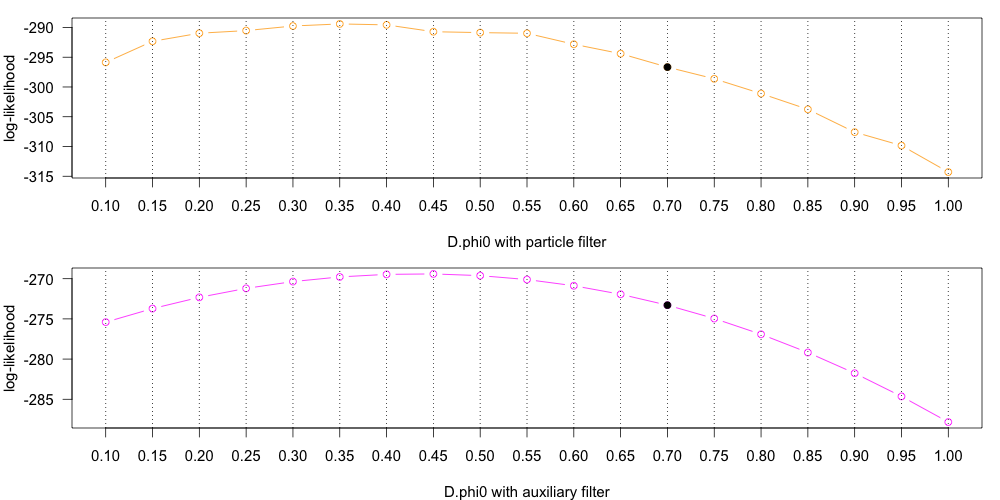
\includegraphics[width=70mm]{../../images/hdpm-loglik-Dphi0.png}
\end{subfigure}%
\begin{subfigure}{.5\textwidth}
  \centering
  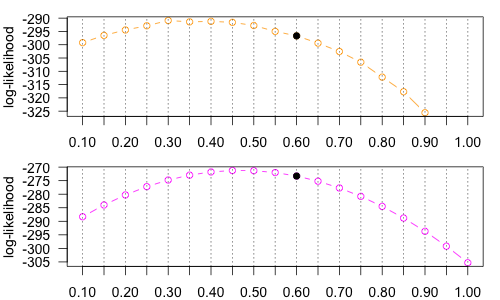
\includegraphics[width=70mm]{../../images/hdpm-loglik-Dphi1.png}
\end{subfigure}
\caption{Belief convergence without misinformation after 300 and 2000 iterations}
\label{fig:conv_nomisinfo}
\end{figure}





%%%%%%%%%%
%    Conclusion   %
%%%%%%%%%%
\chapter{Conclusion}
\label{chp:conclusion}


%%%%%%%%%%%
%    Bibliography          %
%%%%%%%%%%%
%\afterpage{\blankpage}
\nocite{*}
\bibliography{references}
\bibliographystyle{plain}
\end{document}  















